\documentclass[11pt, a4paper]{scrartcl}

\usepackage{listings}
\usepackage{jlcode}
\usepackage{color}
\usepackage[utf8]{inputenc}
\usepackage{hyperref}
\usepackage{graphicx}

\title{Julia Installationsanleitung für Windows}
\author{}
\date{}

\definecolor{dkgreen}{rgb}{0,0.6,0}
\definecolor{dkblue}{rgb}{0,0,0.4}
\definecolor{gray}{rgb}{0.5,0.5,0.5}
\definecolor{mauve}{rgb}{0.58,0,0.82}

\hypersetup{
    colorlinks=true,
    linkcolor=black,
    urlcolor=dkblue,
}
\lstset{
	language=Julia,
%	frame=tb,
	aboveskip=3mm,
	belowskip=3mm,
	showstringspaces=false,
	columns=flexible,
	basicstyle={\small\ttfamily},
	numbers=none,
	numberstyle=\tiny\color{gray},
	keywordstyle=\color{blue},
	commentstyle=\color{dkgreen},
	stringstyle=\color{mauve},
	breaklines=true,
	breakatwhitespace=true,
	tabsize=3
}



\begin{document}
	\maketitle
	
	
	
	
	
	
	\section{Julia herunterladen und installieren}
%	\href{http://julialang.org}{julialang.org}
%	\url{http://julialang.org}
	Öffnen Sie die Webseite \url{https://julialang.org/downloads/} in ihrem Browser. Klicken Sie dort auf den ersten Link mit der Bezeichnung \texttt{64-bit}, um die Julia Installationsdatei herunterzuladen.
	
	\begin{figure}[h!]
		\centering
		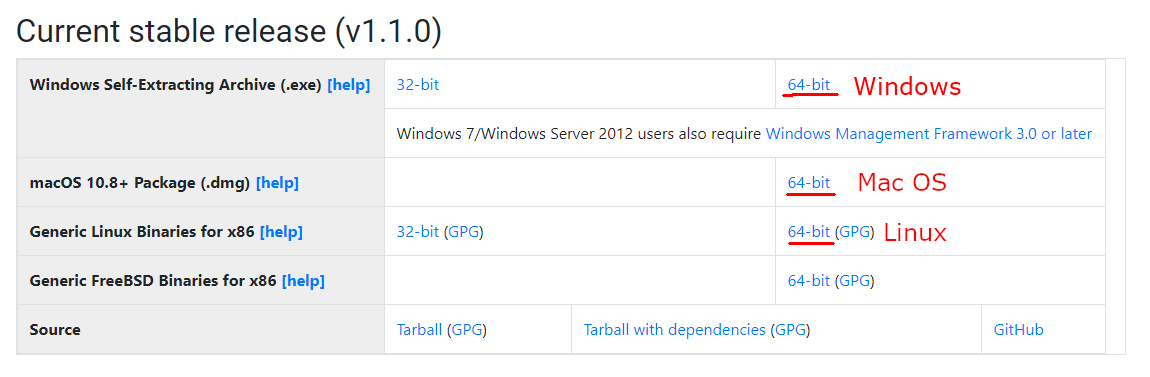
\includegraphics[width=\textwidth]{imgs/download.png}
	\end{figure}

	Führen Sie die heruntergeladene Datei aus. Es sollte nach einem Ladebalken folgendes Fenster erscheinen (eventuell ist der Dialog bei Ihnen auf Deutsch):
	
	\begin{figure}[h!]
		\centering
		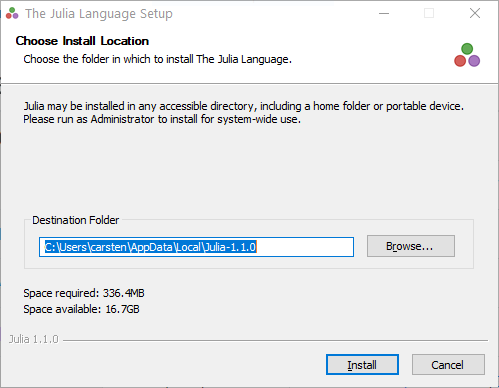
\includegraphics[width=0.5\textwidth]{imgs/install.png}
	\end{figure}

	Klicken Sie auf \texttt{Install}, um Julia zu installieren. Nach Abschluss der Installation erscheint folgender Dialog: 
	

	\begin{figure}[h!]
	\centering
	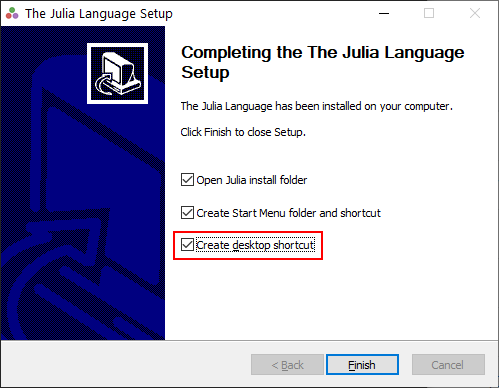
\includegraphics[width=0.5\textwidth]{imgs/install_finish.png}
	\end{figure}

	Setzen Sie beim dritten Auswahlpunkt \texttt{Create desktop shortcut} einen Haken, damit eine Julia Verknüpfung auf dem Desktop erstellt wird. Schließen Sie die Installation mit einem Klick auf \texttt{Finish} ab.
	
	
	
	
	
	
	
	
	
	
	
	
	
	
	
	
	\newpage
	\section{Das erste Mal Julia}
	Starten Sie Julia durch einen Doppelklick auf das Julia Logo auf Ihrem Desktop (oder alternativ über das Windows-Startmenü). Es erscheint das folgende Fenster:
	
	\begin{figure}[h!]
	\centering
	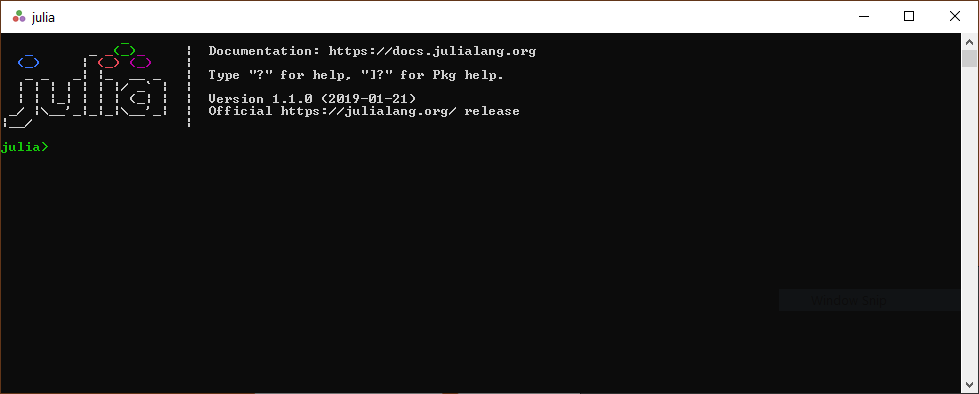
\includegraphics[width=\textwidth]{imgs/julia_REPL.png}
	\end{figure}

	Dies ist die Julia Konsole (auch Julia REPL genannt). Sie ist eine Möglichkeit Julia zu verwenden. Geben Sie zum Test
	
	\begin{lstlisting}
		3+3
	\end{lstlisting}
	
	ein und führen Sie den Befehl per \texttt{Enter}-Taste aus. Sie sollten nicht überraschend das Ergebnis 6 erhalten.
	
	\vspace{1cm}
	
	Auch wenn die Konsole prinzipiell genügt um in Julia zu Programmieren, ist sie doch sehr rudimentär. Im folgenden wollen wir eine viel schickere und Benutzerfreundlichere Julia Oberfläche installieren.
	
	
	
	
	
	
	
	
	
	
	
	\newpage
	\section{IJulia installieren}
	
	Zusätzlich zur Programmiersprache Julia wollen wir noch IJulia und Jupyter installieren, um Julia bequem im Browser in sogenannten Notebooks verwenden zu können. Grob gesagt ist Jupyter eine Notebook Oberfläche für verschiedene Programmiersprachen und IJulia die Schnittstelle zwischen Julia und Jupyter. 
	
	
	Zunächst werden wir in dieser Sektion IJulia installieren. Führen Sie folgenden Befehl in der Julia Konsole aus, indem Sie ihn abtippen (Kopieren und Einfügen ist in der Julia Konsole nicht ganz einfach) und mit der \texttt{Enter}-Taste bestätigen.
	
	\begin{lstlisting}
		using Pkg; Pkg.add("IJulia");
	\end{lstlisting}

	Sie sollten folgende Ausgabe erhalten (die Dateipfade können abweichen):
	
	\begin{figure}[h!]
	\centering
	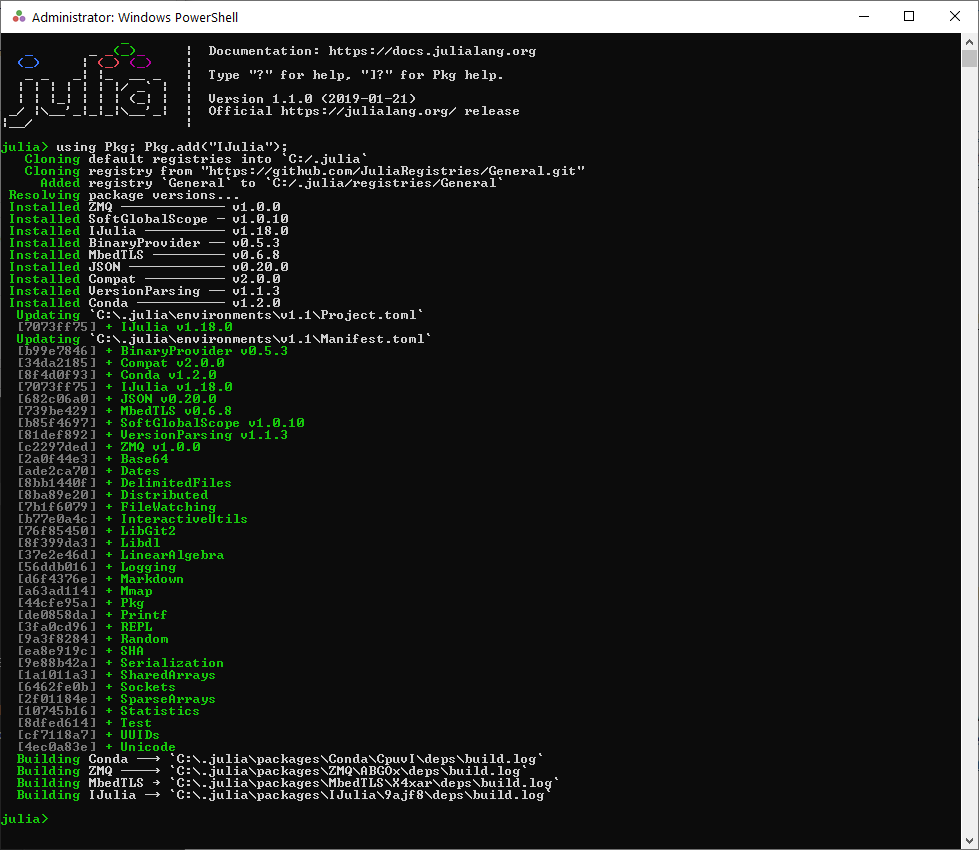
\includegraphics[width=0.9\textwidth]{imgs/IJulia_install.png}
	\end{figure}

	IJulia ist nun erfolgreich installiert.
	
	
	
	
	
	
	
	
	
	
	
	
	
	\section{Jupyter installieren und das erste Mal starten}
	
	Um Notebooks erstellen oder öffnen zu können, muss grundsätzlich zuerst immer Julia geöffnet, IJulia geladen und dann der Jupyter Notebook Server gestartet werden. Im Folgenden wird der erstmalige Vorgang beschrieben, der auch die automatische Installation von Jupyter beinhaltet. 
	
	Stellen Sie sicher, dass Sie eine Julia Konsole geöffnet haben (Dies sollte nach dem vorangegangenen Abschnitt noch der Fall sein, falls nicht öffnen Sie sie erneut per Doppelklick auf das Julia Logo auf dem Desktop) und führen Sie darin folgenden Befehl aus:
	
	\begin{lstlisting}
	using IJulia; notebook()
	\end{lstlisting}
	
	Der erste Teil, \texttt{using IJulia}, lädt IJulia. Der zweite Teil des Befehls, \texttt{notebook()}, versucht den Jupyter Notebook Server zu starten. Julia wird feststellen, dass dieser beim ersten Start noch nicht installiert ist, und fragt uns, ob es Jupyter für uns installieren soll:
	
	\begin{figure}[h!]
	\centering
	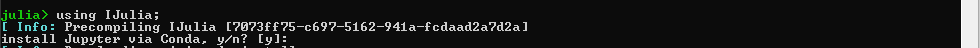
\includegraphics[width=0.9\textwidth]{imgs/Jupyter_install.png}
	\end{figure}
	
	Dies bestätigen wir mit einem Druck der \texttt{Enter}-Taste. Die Installation von Jupyter kann einige Minuten in Anspruch nehmen.
	
	Nach Abschluss der Installation sollte sich automatisch der Browser öffnen und das Jupyter Notebook Interface erscheinen (Ordner, Dateien und Sprache können abweichen):
	
	\begin{figure}[h!]
	\centering
	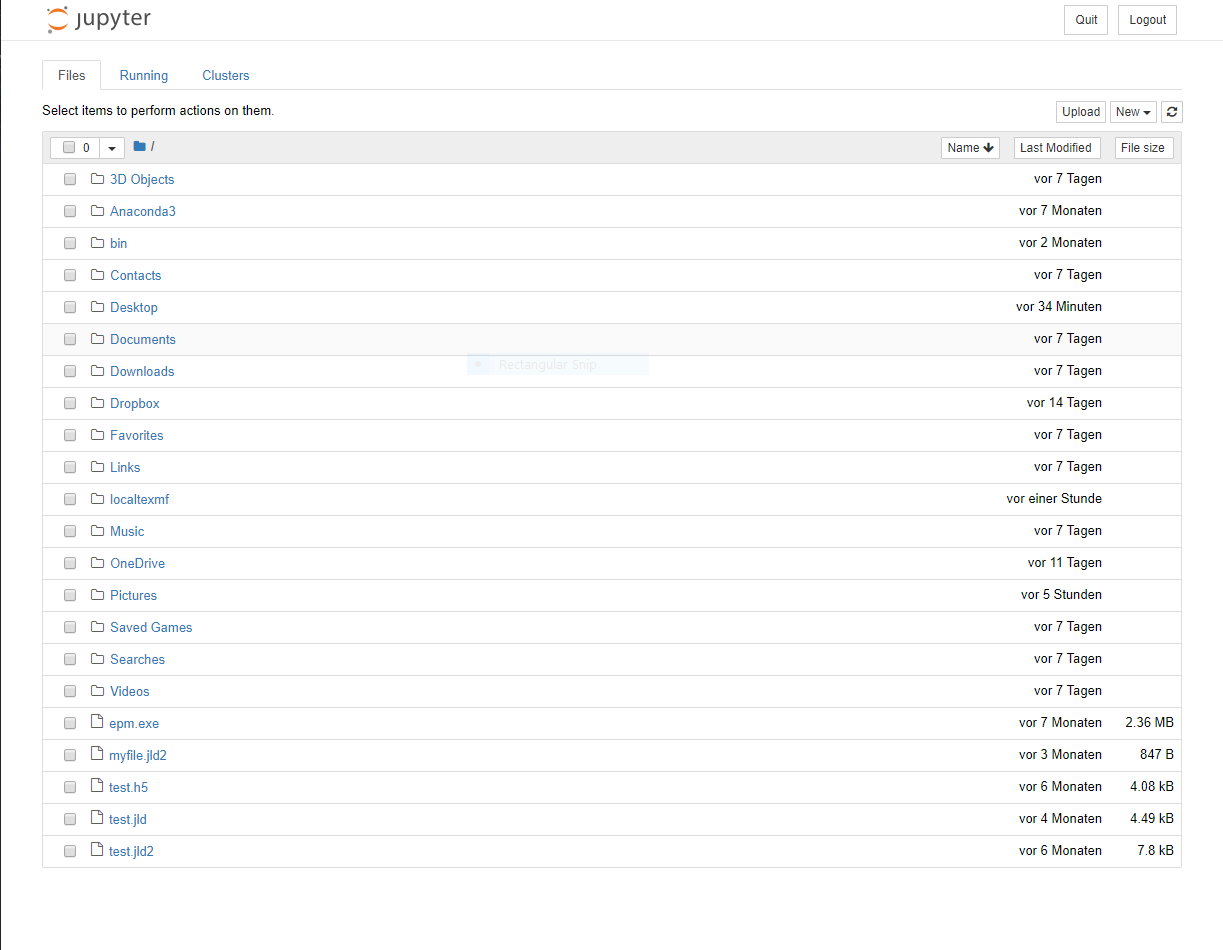
\includegraphics[width=0.6\textwidth]{imgs/jupyter.png}
	\caption{Die Startseite des Jupyter Interfaces. \label{fig:jupyter}}
	\end{figure}
	
	Der Server läuft solange die Julia Konsole im Hintergrund geöffnet ist. Sobald wir diese schließen wird der Server gestoppt.
	
	
	
	
	
	
	
	
	
	
	
	
	
	\newpage
	\section{Einfacher Test der Notebook Oberfläche}
	
	Klicken Sie in der Jupyter Oberfläche (Fig. \ref{fig:jupyter}) rechts oben auf den Button \texttt{New} und klicken Sie danach im sich öffnenden Kontextmenü auf den Eintrag \texttt{Julia 1.1.0}. Es sollte sich nun ein frisches Jupyter Notebook öffnen:
	
	\begin{figure}[h!]
	\centering
	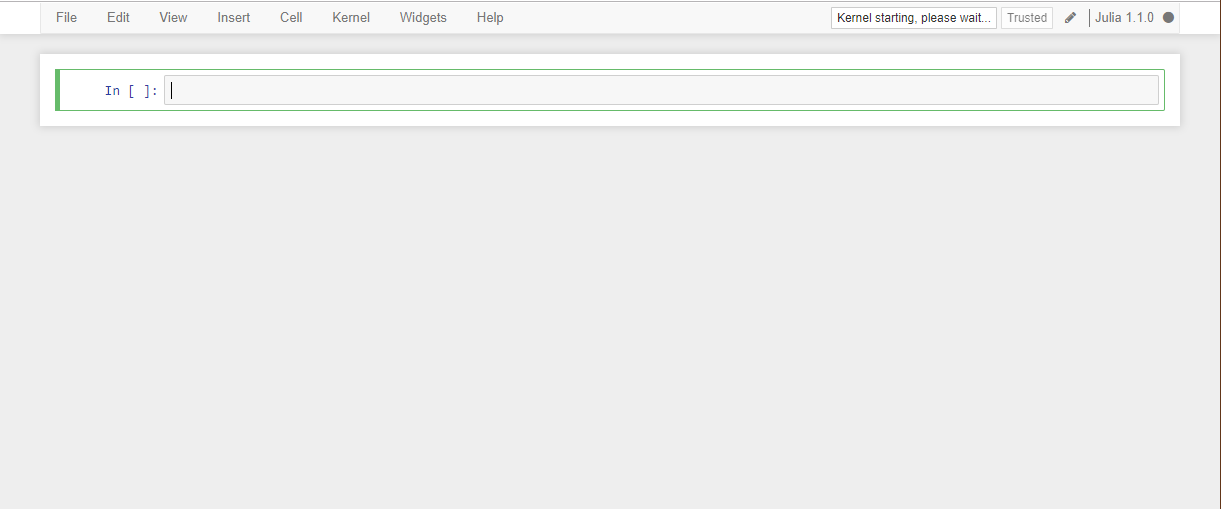
\includegraphics[width=0.9\textwidth]{imgs/jupyter_notebook.png}
	\end{figure}

	Klicken Sie in die erste (und einzige) Zelle des Notebooks und geben Sie dort
	
	\begin{lstlisting}
	3+3
	\end{lstlisting}
	ein. Führen Sie die Zelle per \texttt{SHIFT + ENTER} aus (gleichzeitiges Drücken der \texttt{SHIFT} bzw. \texttt{UMSCHALT} und der \texttt{ENTER} Taste). Es sollte das Ergebnis \texttt{6} erscheinen:

	\begin{figure}[h!]
	\centering
	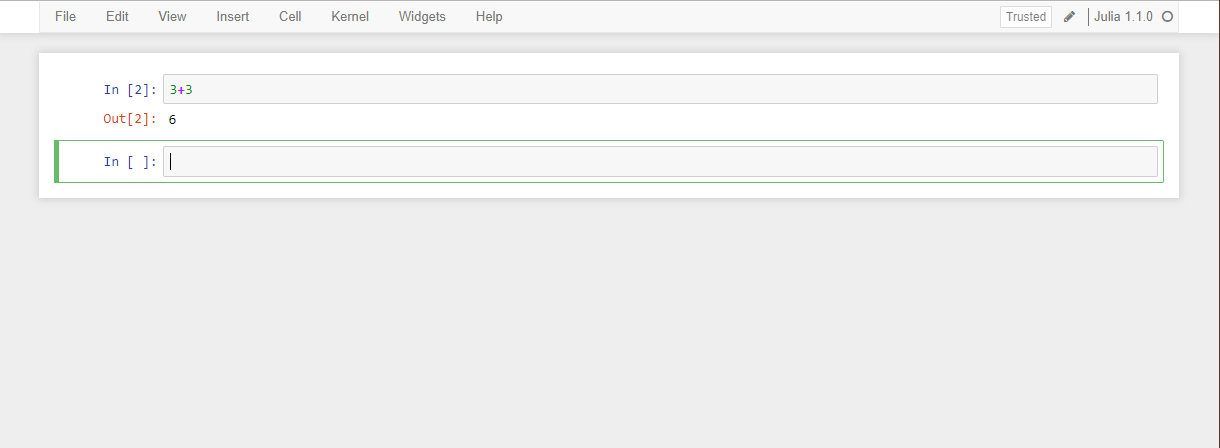
\includegraphics[width=0.9\textwidth]{imgs/jupyter_notebook_test.png}
	\end{figure}	

	Die Installation von Julia, IJulia und Jupyter war also erfolgreich und die Computer-Physik kann beginnen!
	
\end{document}